\section*{Step 4}

\begin{custombox}[label={box:Q4}]{Step 4}
	In each of the above cases generate, capture, and save all the results, for all the datasets, into a common csv file – to facilitate analysis later on. The following metrics (for train and test data) should be created: (For example, see the image that follows):

    \begin{itemize}
        \item Accuracy, Precision (per class), Precision (average), Recall (per class), Recall (average), F1-score (per class), F1-score (average), AUC (per class), AUC (average). 
        \item \textbf{Hint}: The following functions may be used: \texttt{accuracy\_score}, \texttt{precision\_score}, \texttt{recall\_score}, \texttt{f1\_score}, \texttt{roc\_auc\_score}, \texttt{roc\_curve}.
    \end{itemize}

    \begin{figure}[H]
        \centering
        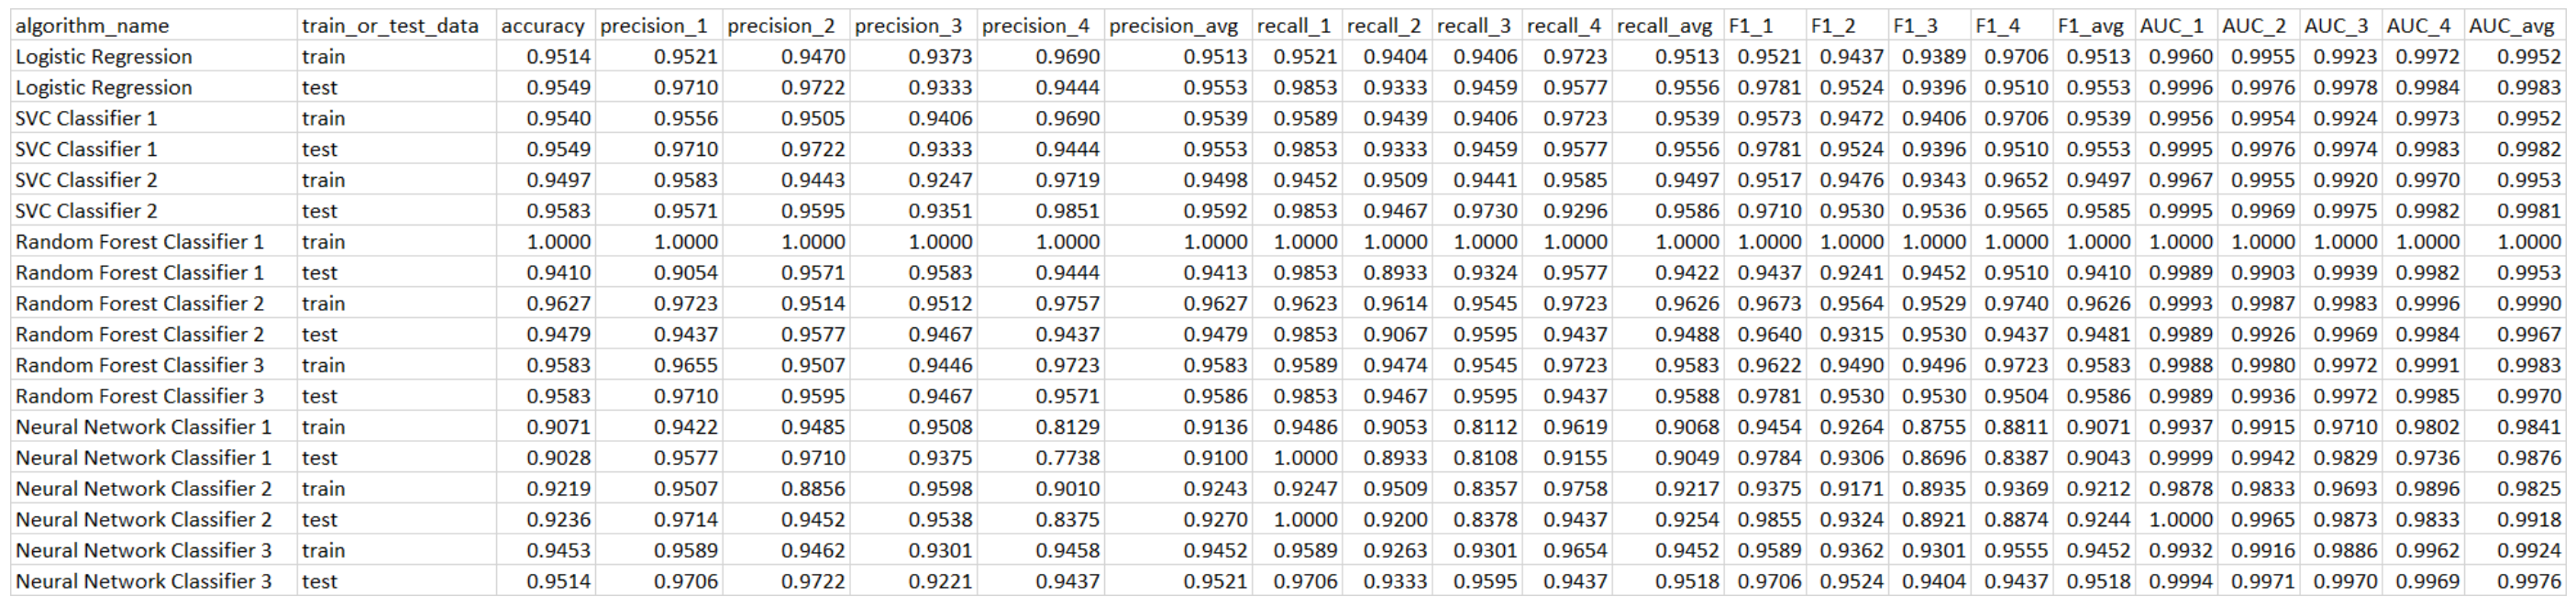
\includegraphics[width=\textwidth]{Images/Step-4-example.png}
        \caption{Example of the CSV file}
        \label{fig:Q4}
    \end{figure}
\end{custombox}

\vspace{5mm}

We define 2 functions: \texttt{get\_metrics} and \texttt{get\_metrics\_df}. The former function calculates the metrics for a given set of true labels, predicted labels, and predicted probabilities. The latter function calculates the metrics for a given dataset and a set of classifiers. We then iterate over all datasets and generate the metrics for each dataset and save them in separate CSV files.

\clearpage

\begin{lstlisting}[language=Python, caption=Generating metrics for all datasets and save them in CSV files, label={lst:Q4}]
def get_metrics(y_true, y_pred, y_prob):
    report = classification_report(y_true, y_pred, output_dict=True)
    acc = accuracy_score(y_true, y_pred)
    
    precisions = [report[f'{i+1}']['precision'] for i in range(4)]
    recalls = [report[f'{i+1}']['recall'] for i in range(4)]
    f1s = [report[f'{i+1}']['f1-score'] for i in range(4)]
    
    aucs = roc_auc_score(pd.get_dummies(y_true), y_prob, multi_class='ovr', average=None)
    
    precision_avg = sum(precisions) / 4
    recall_avg = sum(recalls) / 4
    f1_avg = sum(f1s) / 4
    auc_avg = sum(aucs) / 4
    
    return [acc, *precisions, precision_avg, *recalls, recall_avg, *f1s, f1_avg, *aucs, auc_avg]

def get_metrics_df(data, classifiers):
    x_train, x_test, y_train, y_test = train_test_split(data[['x1', 'x2']], data['y'], test_size=0.2, random_state=42)
    metrics = []

    for name, clf in classifiers.items():
        clf.fit(x_train, y_train) 
        y_train_pred = clf.predict(x_train)
        if hasattr(clf, 'predict_proba'):
            y_train_prob = clf.predict_proba(x_train)
        else:
            decision_values = clf.decision_function(x_train)
            y_train_prob = (decision_values - decision_values.min()) / (decision_values.max() - decision_values.min())
        
        train_metrics = get_metrics(y_train, y_train_pred, y_train_prob)

        y_test_pred = clf.predict(x_test)
        if hasattr(clf, 'predict_proba'):
            y_test_prob = clf.predict_proba(x_test)
        else:
            decision_values = clf.decision_function(x_test)
            y_test_prob = (decision_values - decision_values.min()) / (decision_values.max() - decision_values.min())
        
        test_metrics = get_metrics(y_test, y_test_pred, y_test_prob)
        metrics.append([name, 'train', *train_metrics])
        metrics.append([name, 'test', *test_metrics])
    
    columns = ['algorithm_name', 'train_or_test_data', 'accuracy',
               'precision_1', 'precision_2', 'precision_3', 'precision_4', 'precision_avg',
               'recall_1', 'recall_2', 'recall_3', 'recall_4', 'recall_avg',
               'f1_1', 'f1_2', 'f1_3', 'f1_4', 'f1_avg',
               'auc_1', 'auc_2', 'auc_3', 'auc_4', 'auc_avg']
    
    ret = pd.DataFrame(metrics, columns=columns)
    
    return ret

for i, (data, label) in enumerate(datasets):
    metrics_df = get_metrics_df(data, classifiers)
    metrics_df.to_csv(f'Metrics/metrics-{i+1}.csv', index=False)
\end{lstlisting}

\begin{remark*}
    The CSV files generated in this step can be found in the \texttt{Metrics} directory. The names of the files are \texttt{metrics-1.csv}, \texttt{metrics-2.csv} and \texttt{metrics-3.csv} for datasets 1, 2, and 3 respectively.
\end{remark*}

\clearpage

\subsection*{Various Metrics}

Some of the metrics calculated in this step are as follows:

\begin{itemize}
    \item \textbf{Accuracy}: The proportion of correctly classified instances. This is calculated as 
    \[
        \frac{TP + TN}{TP + TN + FP + FN}
    \]
    \item \textbf{Precision}: The proportion of correctly classified positive instances out of all instances classified as positive. This is calculated as 
    \[
        \frac{TP}{TP + FP}
    \]
    \item \textbf{Recall}: The proportion of correctly classified positive instances out of all actual positive instances. This is calculated as 
    \[
        \frac{TP}{TP + FN}
    \]
    \item \textbf{F1-Score}: The harmonic mean of precision and recall. This is calculated as 
    \[
        2 \times \frac{\text{Precision} \times \text{Recall}}{\text{Precision} + \text{Recall}}
    \]
    \item \textbf{AUC}: The area under the ROC curve. This is calculated using the trapezoidal rule.
\end{itemize}

where:
\begin{align*}
    TP &= \text{True Positives} \\
    TN &= \text{True Negatives} \\
    FP &= \text{False Positives} \\
    FN &= \text{False Negatives}
\end{align*}

\clearpage

